\documentclass[12pt, oneside]{report}
\usepackage{amsmath}
\usepackage{datetime}
\usepackage{todonotes}
\usepackage{amsfonts}
\usepackage{subfiles}
\usepackage[toc, page]{appendix}
\usepackage{tikz,fullpage}
\usepackage[export]{adjustbox}
\usepackage{pgfplots}
\usepackage{footnote}
\usepackage{enumitem}
\usetikzlibrary{tikzmark}
\usepackage{parskip}
\usepackage{amsthm}
\usepackage{listings}
\usepackage{mdframed}
\usepackage[ruled,vlined]{algorithm2e}
\usepackage{subcaption}
\usepackage{multirow}


\usepackage{adjustbox}
\usepackage[backend=biber, style=bibstyle/lncs]{biblatex}
\addbibresource{sources.bib}
\renewcommand{\familydefault}{\sfdefault}
\interfootnotelinepenalty=10000
\usetikzlibrary{arrows.meta}
\usetikzlibrary{arrows, decorations.markings, shapes.geometric}

\tikzstyle{vecArrow} = [thick, decoration={markings,mark=at position
   1 with {\arrow[semithick]{Triangle[open,length=3mm,width=5mm]}}},
   double distance=2.4pt, shorten >= 8pt,
   preaction = {decorate},
   postaction = {draw,line width=2.4pt, white,shorten >= 5pt}]
\theoremstyle{plain}
\newtheorem{thm}{Theorem}[section]
\theoremstyle{definition}
\newtheoremstyle{indented}{3pt}{3pt}{\addtolength{\leftskip}{2.5em}}{
}{\bfseries}{.}{.5em}{}

\theoremstyle{indented}
\newtheorem{defn}[thm]{Definition}
\newtheorem{lemma}[thm]{Lemma}




\newcommand\diag[4]{%
  \multicolumn{1}{p{#2}|}{\hskip-\tabcolsep
  $\vcenter{\begin{tikzpicture}[baseline=0,anchor=south west,inner sep=#1]
  \path[use as bounding box] (0,0) rectangle (#2+2\tabcolsep,\baselineskip);
  \node[minimum width={#2+2\tabcolsep},minimum height=\baselineskip+\extrarowheight] (box) {};
  \draw (box.south west) -- (box.north east);
  \node[anchor=south west] at (box.south west) {#3};
  \node[anchor=north east] at (box.north east) {#4};
 \end{tikzpicture}}$\hskip-\tabcolsep}}

\newenvironment{important}[1][]{%
   \begin{mdframed}[%
      backgroundcolor={red!15}, hidealllines=true,
      skipabove=0.7\baselineskip, skipbelow=0.7\baselineskip,
      splitbottomskip=2pt, splittopskip=4pt, #1]%
   \makebox[0pt]{% ignore the withd of !
      \smash{% ignor the height of !
         \fontsize{32pt}{32pt}\selectfont% make the ! bigger
         \hspace*{-19pt}% move ! to the left
         \raisebox{-2pt}{% move ! up a little
            {\color{red!70!black}\sffamily\bfseries !}% type the bold red !
         }%
      }%
   }%
}{\end{mdframed}}

% Upload fonts and set font families and default
\usepackage{fontspec}
\setromanfont[Ligatures=TeX]{Arial}
\setsansfont[BoldFont=arialnarrowbd.ttf]{arialnarrow.ttf}
\renewcommand{\familydefault}{\rmdefault}

% Set fonts for chapter, section and subsection
\usepackage{titlesec}
\titleformat{\chapter}{\huge\sffamily\uppercase}{\thechapter}{1em}{}

\titleformat{\section}{\normalsize\rmfamily\bfseries}{\thesection}{1em}{}

\titleformat{\subsection}{\normalsize\rmfamily}{\thesubsection}{1em}{}

% Set fonts for in table of contents
\renewcommand{\contentsname}{\uppercase{\sffamily Contents}}



\newcommand{\doctitle}{FPGA-on-FPGA emulation using node disjoint subgraph homeomorphism}
\newcommand{\docsubtitle}{MSc Thesis}
\newcommand{\me}{Pim van Leeuwen}
\newcommand{\studentcode}{s1602772}
\newcommand{\university}{University of Twente}
\newcommand{\school}{EEMCS}
\newcommand{\department}{Formal Methods and Tools}
\newcommand{\supervisor}{dr. W. Kuijper}
\newcommand{\cosupervisor}{dr. ir. R. Langerak}
\newcommand{\cocosupervisor}{H.H. Folmer MSc.}

\author{\me}


\title{FPGA-on-FPGA emulation using vertex disjoint subgraph homeomorphism}
\author{Pim van Leeuwen}
\date{\today}

\begin{document}

\begin{titlepage}
\headheight = 57pt
\footskip = 5pt
\headsep = 0pt


{\begin{Large}
\university\\
\end{Large} }
\school\\
\department\\

\vspace*{5 cm}



\begin{Large}
\textbf{\doctitle}\\
\end{Large}
\docsubtitle\\
\me \quad (\studentcode)\\

\begin{flushright}
\textbf{Technical Supervisor}\\ \supervisor\\
\textbf{Academic Supervisors}\\\cosupervisor\\
\cocosupervisor
\end{flushright}

\vspace*{3cm}
\begin{figure}[h]
\centering
\begin{subfigure}{.5\textwidth}
  \centering
  
\includegraphics[width=.5\linewidth]{images/utwente.png}
\end{subfigure}%
\begin{subfigure}{.5\textwidth}
  \centering
  
\includegraphics[width=.4\linewidth]{images/nedap.png}
\end{subfigure}
\end{figure}





\vfill
\end{titlepage}


\begin{abstract}
FPGAs allow reconfiguration of its logic at any point after production. The result is that they are effective at prototyping application-specific integrated circuits, updating the internal logic while in the field and at low-cost low-quantity use cases. To optimise these processes, it is crucial to properly educate engineers in the implementation of FPGA programs and the FPGA compilation process. Traditional FPGA programming pipelines involve a computationally expensive (NP-hard) place \& route process that slows down iterations of FPGA programs and hinders the educational process. We propose a virtual environment in which place \& route is performed manually in which the student learns about the intricacies of place \& route and in which compilation is linear. To this end, we require emulation of a virtual FPGA on a physical, concrete FPGA. In the proposed research, we find such an emulation using an algorithm that solves a variant of subgraph isomorphism. This algorithm aims to find emulations in as many cases as possible. The expected result is a software package that computes emulators: programs whose output is a program for a concrete FPGA that emulates the provided input program for the virtual FPGA.
\end{abstract}

\newpage
\tableofcontents
\section{Introduction}

\section{Background}
\subsection{Field Programmable Gate Arrays}
\subsubsection{Lookup tables}
\subsubsection{Registers}
\subsubsection{Logic Cells}
\subsubsection{Routing}
\subsubsection{Compilation}
\subsection{Simulation versus Emulation}
\subsection{Path subgraph isomorphism}
\chapter{Objectives}
\label{sec:Objectives}
This research involves how to emulate a virtual FPGA on a concrete FPGA. To this purpose, we have established the following research question:

Given a graph specification of the structural layout of a virtual FPGA $A$ and a graph specification of the structural layout of a concrete FPGA $B$, how do you assemble a linear\footnote{i.e. a numeric constant $c$ exist such that the number of instructions required in the execution of $f$ is less than $c * (\text{the number of configurable components of the virtual FPGA})$. Note that this depends on the size of the \textit{unconfigured} virtual FPGA, not on the size of the user-provided configuration of said FPGA.} function $f$ such that for any representative model of a program $x$ for model A, $f(x)$ is a representative model of a program for model B that is semantically equivalent?
\section*{Subquestion 1}
How do the computational- and space requirements of the generation (not execution) of $f$ scale with the size of FPGAs A and B?
\section*{Subquestion 2}
How much wiring and how many components does the concrete FPGA need for emulation of a virtual FPGA of complexity $x$? Is this practical for use in education?
\section*{Expected outcomes}
We expect an algorithm and an implementation of that algorithm that, given models of both a virtual FPGA and a (larger) concrete FPGA, generates a function that translates a model of an FPGA program compatible with the virtual FPGA to a model of an FPGA program compatible with the concrete FPGA. We generalise this algorithm to other use cases with the same underlying mathematical problem (subgraph homeomorphism). Furthermore, we include specifications on how to model FPGA models for this purpose. 
\section{Models}
\subsection{FPGA}
Our algorithm will generate an emulation using path subgraph isomorphism. To this end, we will model FPGA designs as graphs. For this purpose, let us define the type $hierarchygraph : (V, E, L, H)$ where $V$ is a set of vertices, $E\subseteq (V \times V)$ is a set of undirected edges, $L$ is a vertex labeling function $V \to \lambda$ where $\lambda$ is a finite set of labels and $H$ describes the hierarchy with a relation $V \to hierarchygraph$. We restrict ourselves to graphs without loops, i.e. $\not \exists v \in V . (v, v) \in E$. Let $model(B)$ be the $hierarchygraph$ model of (a subset of) an FPGA layout $B$. Then:

\begin{itemize}
\item Whenever $B$ has a connection to external hardware (e.g. a pin) with an optional identifier $k$ where order is relevant, $model(B)$ has an edge to a distinct vertex $v$ and $L(v)=``port\_out_k"$.

\item Each component that is one step lower than $B$ in the FPGA hierarchy (e.g. CLBs) corresponds to a distinct vertex $v$ such that $L(v)=``component"$ and with a set of vertices $S$ with optional identifiers such that $\forall s \in S . L(s)=``port\_in_{id(s)}" \land (s,v) \in E$. Furthermore, the contents of this component are recursively defined in $H(v)$.

\item Whenever $B$ has a routing switch, $model(B)$ has a distinct vertex $v$ and $L(v)=``switch"$.

\item Whenever $B$ has a mux with $n$ wires for each input and for its output, $model(B)$ has distinct vertices $\{v_{left, 1} \dots v_{left, n}\} \cup \{v_{right, 1} \dots v_{right, n}\} \cup \{v_{out, 1} \dots v_{out, n}\} \cup \{v_{select}\}$ where:

\begingroup
\setlength{\tabcolsep}{2pt} % Default value: 6pt
\begin{tabular}{llllll}
$\forall v_{left, i}$ & $\in \{v_{left, 1} \dots v_{left, n}\}$ & $. L(v_{left, i}$&$= ``mux\_left_i"$&$\land (v_{left, i}$&$, v_{select}) \in E$,\\
$\forall v_{right, i}$ & $\in \{v_{right, 1} \dots v_{right, n}\}$ & $. L(v_{right, i})$&$= ``mux\_right_i"$&$\land (v_{right, i}$&$, v_{select}) \in E$,\\
$\forall v_{out, i}$ & $\in \{v_{out, 1} \dots v_{out, n}\}$ & $. L(v_{out, i}) $&$= ``mux\_out_i"$&$\land (v_{out, i}$&$, v_{select}) \in E$ and
\end{tabular}
\endgroup

$L(v_{select})=``mux\_select"$

Whenever something is connected to input or output of the mux in $B$, $model(B)$ has an edge to the corresponding vertex $v \in \{v_{left, 1} \dots v_{left, n}\} \cup \{v_{right, 1} \dots v_{right, n}\} \cup \{v_{out, 1} \dots v_{out, n}\}$. Furthermore, if $B$ has a wire to the selection input, $model(B)$ has an edge to the vertex $v_{select}$.

\item Each LUT that has $n$ inputs and $m$ outputs corresponds to\todo{change to $model(B)$} unique vertices $v_{in}$ and $v_{out}$ such that $L(v_{in})=``lut_{in}"$, $L(v_{out})=``lut_{out}"$ and $(v_{in}, v_{out}) \in E$. Wires to the input of the LUT correspond with edges to $v_{in}$ whilst wires from the output of the LUT correspond with edges from $v_{out}$.

\item Each register that has $n$ inputs corresponds\todo{change to $model(B)$} to:

$\{v_{in, 1} \dots v_{in, n}\} \cup \{v_{out, 1} \dots v_{out, n}\} \cup \{v_{set}, v_{resetsync}, v_{resetasync}\}$ where

\begingroup
\setlength{\tabcolsep}{2pt} % Default value: 6pt
\begin{tabular}{llllll}
$\forall v_{in, i}$ & $\in \{v_{in, 1} \dots v_{in, n}\}$ & $. L(v_{in, i})$&$=``register\_in_i"$&$\land (v_{in, i}, v_{set})$&$\in E$, \\
$\forall v_{out, i}$ & $\in \{v_{out, 1} \dots v_{out, n}\}$ & $. L(v_{out, i})$&$=``register\_out_i"$&$\land (v_{out, i}, v_{set})$&$\in E$, \\
\end{tabular}
\endgroup

$L(v_{set})=``register\_set"$,

\begingroup
\setlength{\tabcolsep}{2pt} % Default value: 6pt
\begin{tabular}{llll}
$L(v_{resetsync})$&$=``register\_reset\_sync"$&$\land (v_{set}, v_{resetsync}) $&$\in E$ and\\
$L(v_{resetasync})$&$=``register\_resFet\_async"$&$\land (v_{set}, v_{resetasync}) $&$\in E$.
\end{tabular}
\endgroup

A connection to an input of the register at wire position $x$ corresponds with\todo{change to $model(B)$} an edge to $v_{in, x}$. Similarly, a connection to an output of the register at wire position $x$ corresponds with\todo{change to $model(B)$} an edge to $v_{out, x}$. Connections to the set-, synchronous reset and asynchronous reset gates in the FPGA correspond to\todo{change to $model(B)$} edges to the respective vertex in $\{v_{set}, v_{resetsync}, v_{resetasync}\}$.
 

\item Each connection by wire corresponds to\todo{change to $model(B)$} an edge.
\end{itemize}
\subsection{FPGA program}
\section{Algorithm}
\subsection{State space storage}
\subsection{State space exploration}
\subsection{Hierarchy usage}
\subsection{Defining $f$}
\chapter{Pruning}
\label{chapter:pruning}

During the search for a complete matching, during which the algorithm only has \textit{partial} matchings, the algorithm will often explore branches of the search tree that will not eventually lead to a homeomorphism. We will call these branches \textit{dead branches}. Exploring an entire dead branch may be costly: its size is exponential\footnote{due to the NP-completeness of node disjoint subgraph homeomorphism} thus exploration costs an exponential amount of time. A solution to this is to implement methods of early detection of such dead branches, i.e. pruning methods. These methods can by nature not detect every dead branch efficiently\footnote{again, because of the NP-completeness of node disjoint subgraph homeomorphism.}. Therefore, there exists a tradeoff between strength, i.e. how many dead branches it can detect, and performance, i.e. how the number of instructions used by pruning scales with the size of the inputs.

%Various pruning methods for subgraph isomorphism exists [refs]. We write bla for subgraph homeomorphism


%if is isomorphism is homeo but homeo not necc iso

%pruning aan de hand van die invariants


%herschrijf pruning methods
Algorithms for subgraph \textit{isomorphism} use various pruning methods, which we will implement for subgraph \textit{homeomorphism}. Subgraph isomorphism is, however, a stricter problem than subgraph homeomorphism. Each subgraph isomorphism mapping is a node disjoint subgraph homeomorphism but not every subgraph homeomorphism is a subgraph isomorphism. Because of this, its pruning methods can filter away some search tree branches that could never result in a subgraph isomorphism, but that could possibly result in a node disjoing subgraph homeomorphism. This means that possibly fewer dead branches can be pruned in the search for subgraph homeomorphisms compared to subgraph isomorphism. In this research, we will experiment with different pruning methods applied to searching subgraph homeomorphisms and draw conclusions about their applicability.

% 
The input of these pruning methods comes down to an assignment of domains (sets of target graph vertices) to variables (source graph vertices). These domains represent the target graph vertex candidates for each source graph vertex in vertex-on-vertex matching. Source graph vertices that are already in the partial matching have a domain of size one: the target graph vertex they have been matched to. The other vertices have domains that can be calculated in different ways (see Section \ref{sec:domain-filtering}). The pruning method then decides whether the algorithm should continue the search in this branch (i.e. do not prune) or whether the algorithm should backtrack. The different methods of deciding this are elaborated in Section \ref{sec:pruningmethods}.

\section{Domain filtering}
\label{sec:domain-filtering}
The goal of domain filtering during a search is to assign a domain of target graph vertices to each source graph vertex such that the following three criteria are satisfied:

\begin{enumerate}
\item \label{li:complete}If at least one homeomorphism can be found from this search branch, then for some homeomorphism that can be found from this search branch with vertex-on-vertex matching $M_V$ it holds that $\forall (s \to t) \in M_V . t \in \mathit{domain}(s)$.
\item \label{li:falsepositives}Each domain assignment contains as few `false positives' as possible, where a false positive is a pair of a source vertex $s$ and a target vertex $t$ such that $t$ is in the domain of variable $s$ and no homeomorphism exists from the current search path in which $s$ is matched to $t$.
\item \label{li:complexity} The process of domain filtering has a computational complexity that is as low as possible.
\end{enumerate}

In this section, we will explore different methods to obtain these domains, each with different tradeoffs between strength (performing better at criterium \ref{li:falsepositives}) and performance (performing better at criterium \ref{li:complexity}).
\subsection{Labels and neighbours}
The weakest and fastest method to obtain domains for some source graph vertex $u$ is by selecting each unmatched target graph vertex $v$ that has compatible labels and has compatible in- and outdegrees:

\begin{minipage}{\textwidth}
\begin{defn}[compability under label constraint] If $M$ is the current partial matching, then:

\[\mathit{compatible}_{\mathit{LABEL}}(u, v) := v \not \in M \land L(u) \subseteq L(v) \land |\mathit{pred}(v)| \geq |\mathit{pred}(u)| \land |\mathit{succ}(v)| \geq |\mathit{succ}(u)|\]

\end{defn}
\end{minipage}

This method satisfies criterium \label{li:complete} since every homeomorphism needs each source graph vertex $u$ to be matched with a target graph vertex $v$ that has at least the same label set as $u$, and the possibility of connecting with each mapped predecessor and successor of $u$. It has a low computational complexity per source-target pair ($O(|L_S|)$).

\subsection{Free neighbours}
A somewhat stronger and somewhat slower method to obtain domains in addition to label filtering is to compare the indegree- and outdegree of each unmatched source graph vertex $u$ to other unmatched source graph vertices to the in- and outdegree of the target graph vertex $v$ to other unmatched target graph vertices. The target graph vertex must have a larger or equal indegree and outdegree compared to the source graph vertex:


\begin{minipage}{\textwidth}
\begin{defn}[compatibility under free neighbours constraint] If $M$ is the current partial matching, then:

$\mathit{compatible}_{\mathit{FN}}(v,u) := \mathit{compatible}_{\mathit{LABEL}}(v,u) \land C_{\mathit{indegree}}(v, u) \land C_{\mathit{outdegree}}(v, u)$

where:

$C_{\mathit{indegree}}(u, v) := |\{v' \in \mathit{pred}(v) .  v' \not \in M\}| \geq |\{u' \in \mathit{pred}(u) . u' \not \in M\}$

$C_{\mathit{outdegree}}(u, v) := |\{v' \in \mathit{succ}(v) . v' \not \in M\}| \geq |\{u' \in \mathit{succ}(u) . u' \not \in M\}$
 
\end{defn}
\end{minipage}

This method satisfies criterium \label{li:complete} since 


\subsection{Reachability of matched vertices}
A strong (and computationally very expensive) method of filtering the domain we will use\footnote{An even stronger method would be to find paths that each have different second vertices and each have different second-last vertices, or even to check that no intermediate vertex is used multiple times (NP-complete). This is, however, out of scope for this research.} for some source graph vertex $u$ and some target graph vertex $v$ in addition to label- indegree and outdegree compability is to check that $v$ can reach the mapped vertices of successors of $u$ and that $v$ can be reached from the mapped vertices of predecessors of $u$, i.e. that candidate paths exist for the upcoming edge-path matching attempts. This pruning method does not check whether a set of paths exist that is vertex disjoint since that is the task of the main algorithm: it merely checks the existence of paths. If no path exists, then no vertex disjoint path exists and pruning is required. An example of a domain filtered by reachability can be found in Figure \ref{fig:reachability-filtered}. Formally:


\begin{minipage}{\textwidth}
\begin{defn}[compatibility under reachability constraint]

If $M$ is the current partial mapping and $P$ is the set of paths in the target graph, then:

$\mathit{compatible}_{\mathit{REACH}}(v,u) := \mathit{compatible}_{\mathit{FN}}(v,u) \land C_{\mathit{inr}}(v, u) \land C_{\mathit{outr}}(v, u)$

where:

\begin{tabular}{lll}
$C_{\mathit{inr}}(u, v) := \forall u' \in (\mathit{pred}(u) \cap M) .  \exists p \in P .$&$\mathit{first}(p)=M(u')$&$\land$\\
&$\mathit{last}(p)=v$&$\land$\\
&\multicolumn{2}{l}{$\not \exists i \in \mathit{intermediate}(p) . i \in M$}
\end{tabular}

\begin{tabular}{lll}
$C_{\mathit{outr}}(u, v) := \forall u' \in (\mathit{succ}(u) \cap M) .  \exists p \in P .$&$\mathit{first}(p)=v$&$\land$\\
&$\mathit{last}(p)=M(u')$&$\land$\\
&\multicolumn{2}{l}{$\not \exists i \in \mathit{intermediate}(p) . i \in M$}
\end{tabular}
\end{defn}
\end{minipage}



\begin{figure}
\centering
\parbox{1.2in}{

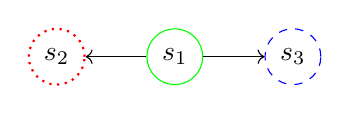
\begin{tikzpicture}

\node[circle, draw=green] at (0,0) (a) {$s_1$};
\node[circle, draw=red, dotted, thick] at (-1.5,0) (b)  {$s_2$};
\node[circle, draw=blue, dashed] at (1.5,0) (c)  {$s_3$};

\draw[->] (a)->(b);
\draw[->] (a)->(c);
\end{tikzpicture}
}
\qquad\qquad
\begin{minipage}{1.2in}%

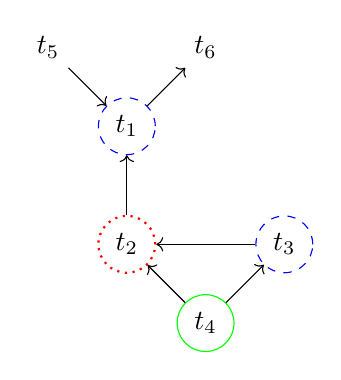
\begin{tikzpicture}
\node[circle, draw=green] at (0,0) (blue) {$t_4$};
\node[circle, draw=red, dotted, thick] at (-1,1) (green) {$t_2$};
\node[circle, draw=blue, dashed] at (1,1) (yellowone) {$t_3$};
\node[circle, draw=blue, dashed] at (-1,2.5) (yellowtwo) {$t_1$};
\node at (-2,3.5) (redone) {$t_5$};
\node at (-0,3.5) (redtwo) {$t_6$};

\draw[->] (blue) -> (green);
\draw[->] (blue) -> (yellowone);
\draw[->] (yellowone) -> (green);
\draw[->] (green) -> (yellowtwo);
\draw[->] (redone) -> (yellowtwo);
\draw[->] (yellowtwo) -> (redtwo);


\end{tikzpicture}
\end{minipage}
\caption{After vertex placements $s_1 \to t_4$ and $s_2 \to t_2$, the domain for vertex $s_3$ would normally be $\{t_1, t_3\}$. However, by checking for reachability from $t_4$ we can reduce this to $\{t_3\}$. The numbers represent the matching order and the circle styles represent labels.}
\label{fig:reachability-filtered}
\end{figure}
\subsection{Reachability of neighbourhood}
In addition to filtering domains based on the current partial matching and the source- and target graph, we can perform domain filtering based on domains that are already computed. If some source graph vertex $s_1$ with domain $D_1$ has an edge to some vertex $s_2$ with domain $D_2$, then for each target graph vertex $t_1 \in D_1$ there must exist a path to some vertex $t_2 \in D_2$. If not, then $t_1$ may be removed from $D_1$. We will call this filtering \textit{level 1 neighbourhood filtering}. If we $D_2$ was itself filtered using level 1 neighbourhood filtering, we call this \textit{level 2 neighbourhood filtering}. Similarly, each additional time the neighbourhood reachability filtered domain is reused in another neighbourhood reachability filtering we consider it of a higher level. When computing domains serially, an appropriate maximum level should be used: using level 2 neighbourhood filtering over level 1 neighbourhood filtering yiels, for example, much more domain reduction and is much less computationally demanding compared to level 20 neighbourhood filtering over level 19 neighbourhood filtering. However, if a cached approach is used (see section TODO), we can perform level $\infty$ neighbourhood filtering using a fixed point algorithm.

\section{Pruning methods}
\label{sec:pruningmethods}
\subsection{ZeroDomain pruning}
%applicable to both isomorphism and homeomorphism
The ZeroDomain pruning method decides to backtrack if and only if one of the domains is empty, i.e. there exists some source graph vertex that cannot be matched with any target graph vertex. A homeomorphism cannot be found in the current search branch as no potential match exists for this source graph vertex. An example of a domain assignment where ZeroDomain prunes the search space is shown in Table \ref{tab:zerodomain}.

\label{sec:emptyDomain}
\begin{table}
\centering
\begin{tabular}{|l|l|}
\hline
\textbf{Source graph vertex} & \textbf{Target graph candidates} \\ \hline
$s_1$                          & $\{t_1, t_3, t_5\}$         \\ \hline
$s_2$                          & $\{t_1, t_2, t_3, t_4\}$       \\ \hline
$s_3$                          & $\{t_2, t_3, t_6\}$      \\ \hline
$s_4$                          & $\emptyset$                      \\ \hline
\end{tabular}
\caption{If the empty domain pruning method detects an empty target graph domain for some source graph vertex, backtracking is initiated. This is the case if the possible target graph candidates are as shown as in this table.}
\label{tab:zerodomain}
\end{table}

\subsection{AllDifferent pruning}
\label{sec:alldifferent}
The AllDifferent constraint specifies that every variable should be able to have a different value. This is the case with some variable having an empty domain (i.e. AllDifferent is stronger than ZeroDomain), but also in other cases. Since a homeomorphism requires such an assignment, the AllDifferent pruning algorithm backtracks in this case. Unfortunately, we could not find an AllDifferent implementation using less than quadratic space. An example of a domain assignment where AllDifferent prunes the search space but ZeroDomain does not is shown in Table \ref{tab:alldifferent}. 

\begin{table}
\centering
\begin{tabular}{|l|l|}
\hline
\textbf{Source graph vertex} & \textbf{Target graph candidates} \\ \hline
$s_1$                          & $\{t_1, t_2, t_3\}$      \\ \hline
$s_2$                          & $\{t_1, t_2\}$              \\ \hline
$s_3$                          & $\{t_2, t_3\}$              \\ \hline
$s_4$                          & $\{t_1, t_3\}$             \\ \hline
\end{tabular}
\caption{In this example, four source graph vertices have a total domain of only three target graph candidates. By the pigeonhole principle, no injective assignment is possible. AllDifferent recognises this and initiates backtracking.}
\label{tab:alldifferent}
\end{table}




\section{When to apply}
When a pruning method has been selected and a strategy to obtain the domains, one must lastly decide when to apply the pruning method.
\subsection{Runtime calculation}
The simplest option is to calculate the domains and run the pruning strategy each time a vertex is selected for usage in a matching. This could be a target graph vertex that is selected as for vertex-on-vertex matching or a target graph vertex that is part of a path in edge-on-path matching. This changes the partial matching and thus the domains. The pruning method then decides to allow it or to disallow it.
\subsection{Caching domains - incremental domain calculation}
Another option is to cache the domain of each variable and update it based on the current partial matching. This saves valuable time but requires quadratic space\footnote{i.e. some constant $c$ exists such that the space required has an upper bound of $c * |V_{target}|^2$} (for each source graph vertex $\in |V_{source}|$ it needs to store a domain of average size $O(|V_{target}|)$). If the reachability pruning method is used, paths need to be cached as well. That is, for each edge $\in E_{source}$ we need to store a path of $O(|V_{target}|)$ vertices.
\subsection{Parallel calculation}
Finally, we can perform the domain filtering and procedure in a seperate CPU thread while the algorithm continues without backtracking. The pruning thread queries the current matching and calculates whether pruning is appropriate for that matching. If it decides that it is not, it requeries the current matching. Otherwise, it will interrupt the main thread and signal it to backtrack until the pruning method does not detect a dead branch anymore. This method cannot perform caching

\chapter{Business case: Lattice ECP5}
We will apply our algorithm to map virtual FPGAs to the concrete Lattice ECP5 FPGA. An image of this FPGA on an evaluation board is shown in Figure \ref{fig:evaluationboard}. This FPGA's architecture consists of `tiles' of different types in a grid pattern. Each of these tiles has an associated x- and y-coordinate in the grid system and is (generally) topologically the same as tiles of the type elsewhere in the grid. There exist I/O tiles which' function is to retrieve and send data from outside the FPGA, DSP tiles that perform signal processing calculations, tiles that only provide routing structure, RAM tiles and tiles that are internally used for clock management and configuration.

\begin{figure}
\centering
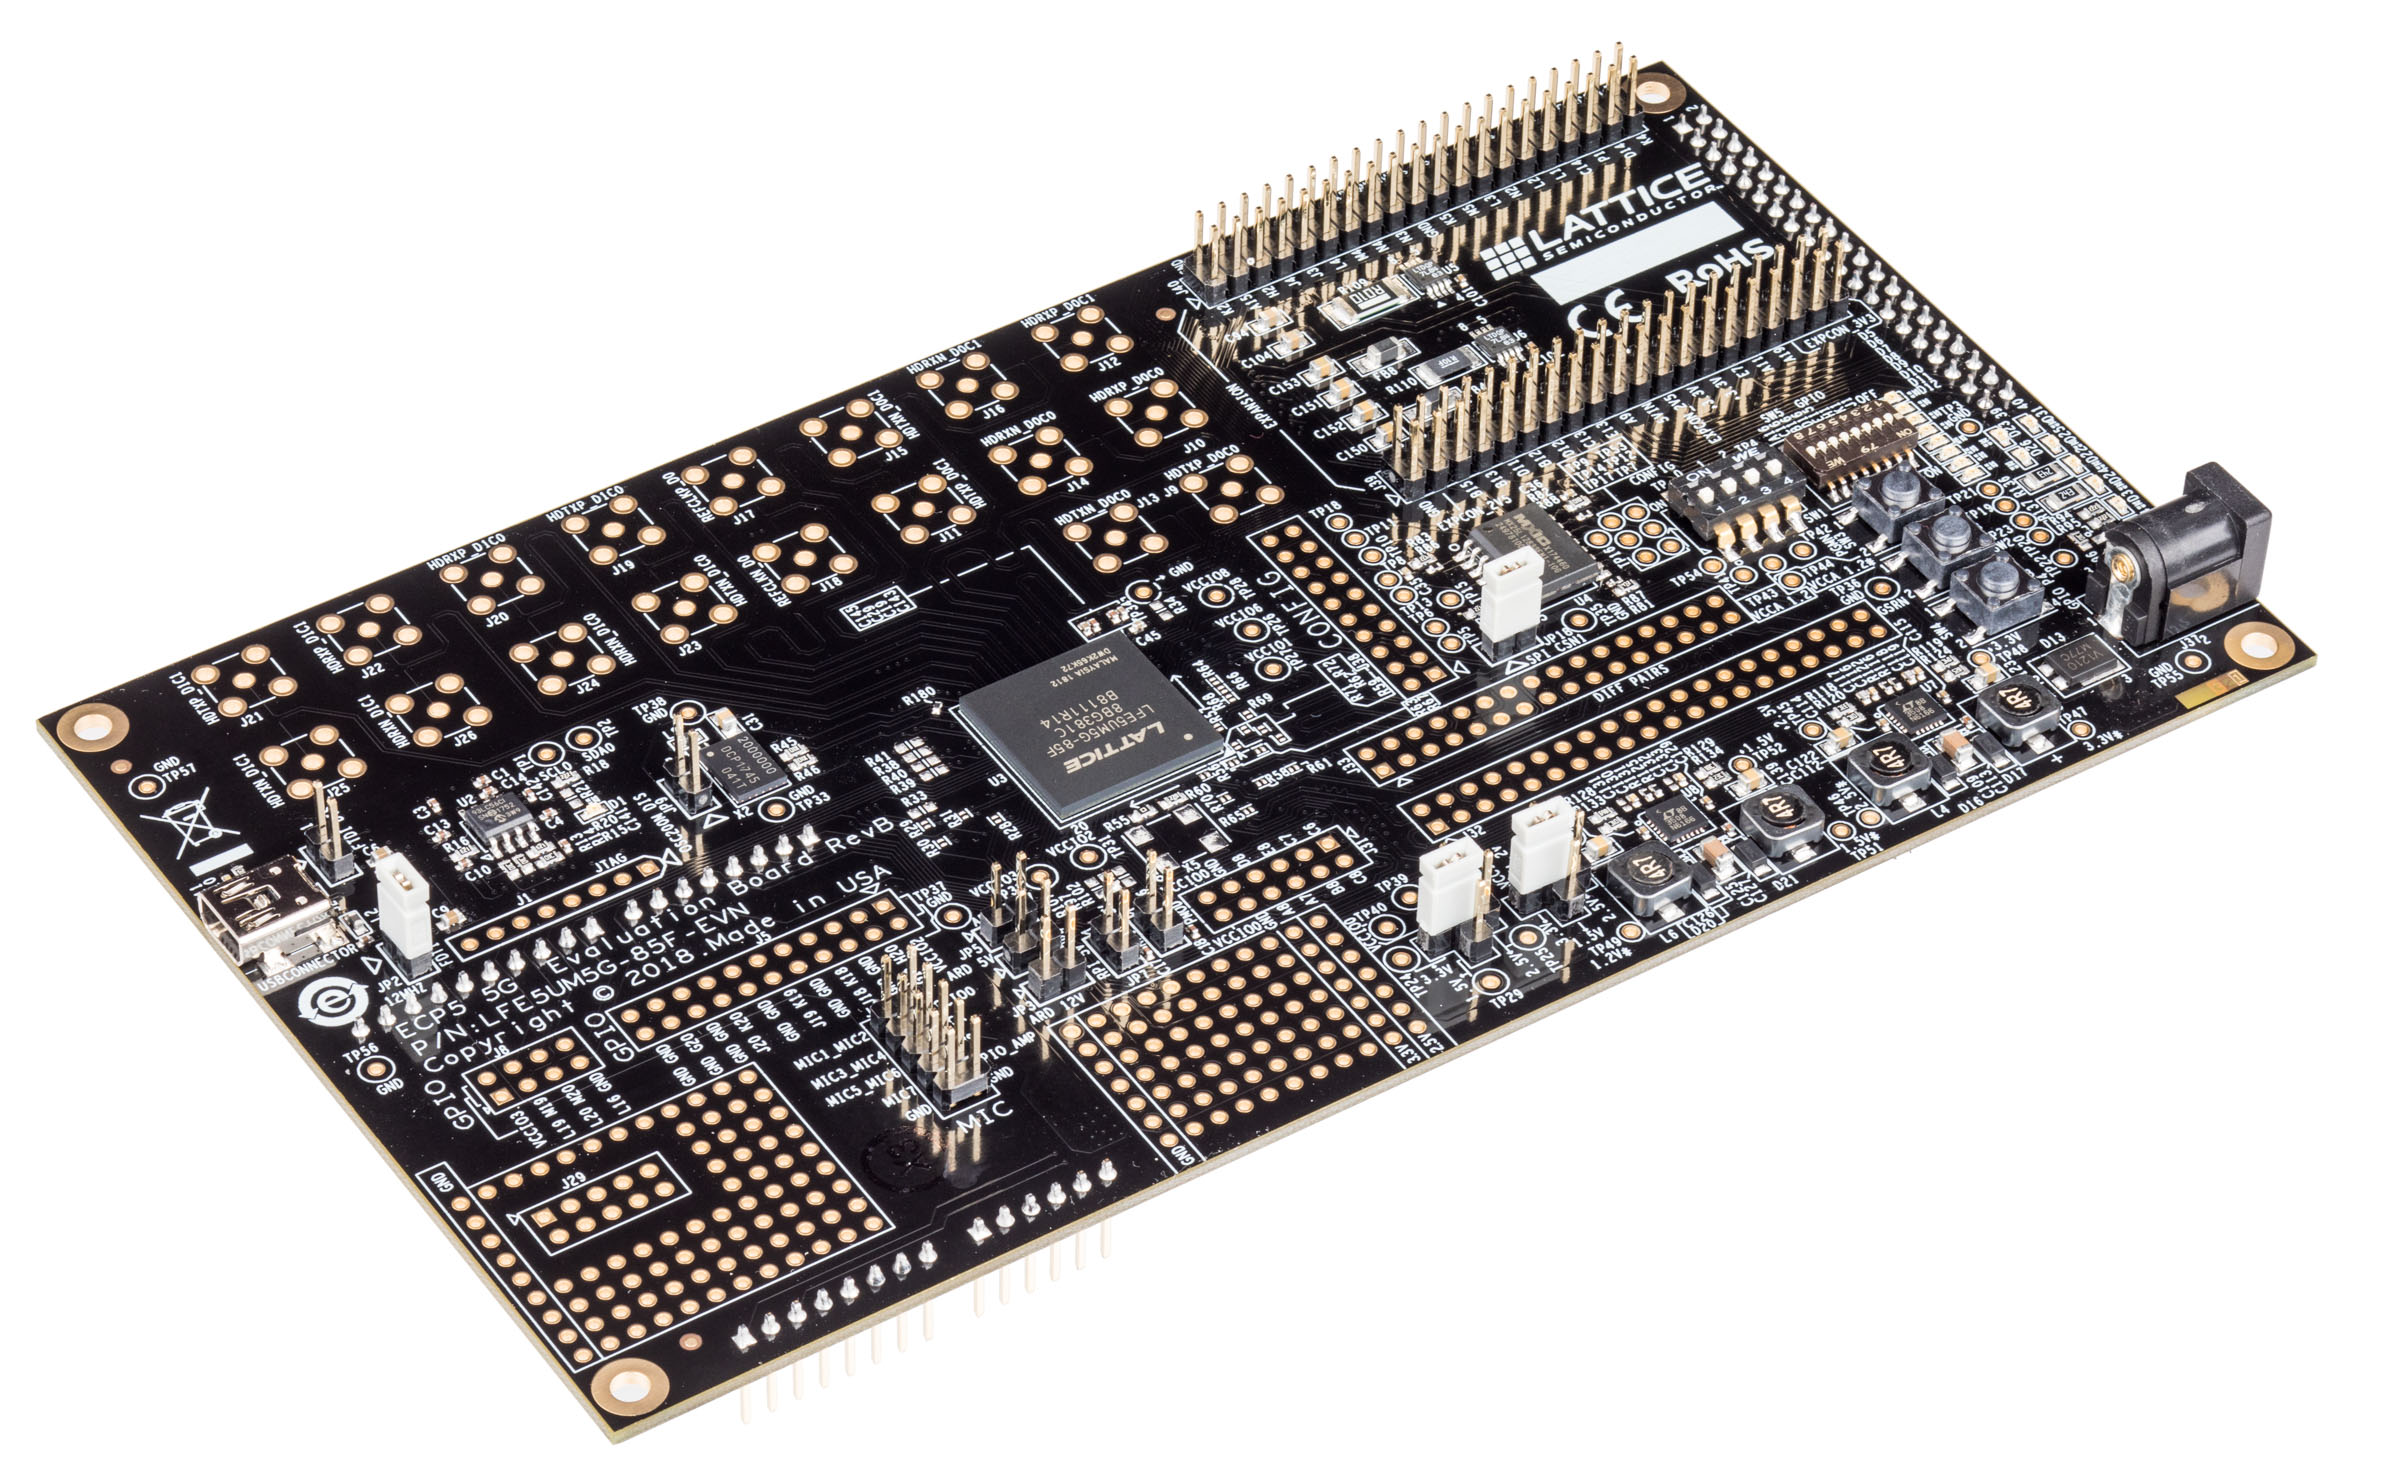
\includegraphics[width=0.5\textwidth]{images/ECP5.png}
\caption[Evaluation board of the LFE5UM5G-85F FPGA: a variant of the ECP5.]{Evaluation board of the LFE5UM5G-85F FPGA: a variant of the ECP5.\footnotemark}
\label{fig:evaluationboard}
\end{figure}
\footnotetext{\texttt{http://www.latticesemi.com/products/developmentboardsandkits/ecp5evaluationboard}, accessed July 10th 2020}	

The structure of an ECP5 FPGA is shown in Figure \ref{fig:ecp5architecture}. This figure shows the grid/tile structure of the ECP5 along with specific components from the electrical engineering domain. The largest portion of the grid structure consists of logic tiles that contain 8 LUTs and 8 registers (or flip-flops (FF)), bundled in 4 modules. We will focus on this type of tile to find homeomorphisms. We used Project Trellis \cite{trellis} to obtain graphs of both an individual tile (shown in Figure \ref{fig:ECPTGephi}) and of collections of adjacent tiles.

\begin{figure}
\centering
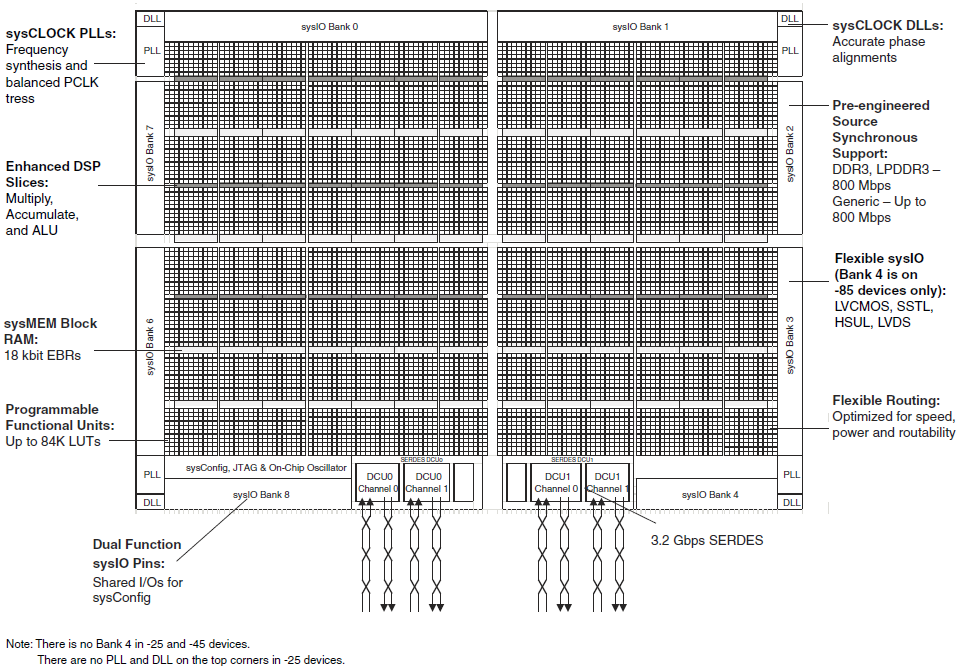
\includegraphics[width=0.8\textwidth]{images/ECP5Architecture.png}
\caption[Architecture of the ECP5 FPGA. Note that it is tile-based in a square grid structure]{Architecture of the ECP5 FPGA. Note that it is tile-based in a square grid structure.\footnotemark}
\label{fig:ecp5architecture}
\end{figure}
\footnotetext{ECP5\texttrademark and ECP5-5G\texttrademark Family Data Sheet (FPGA-DS-02012 Version 1.9), accessed October 1st 2020}	

The virtual FPGA we aim to emulate on this board (which we will call \textit{VirBoard}) is one that, like the ECP5 consists of a tile-like structure with no wires spanning no more than a single tile. Because of this limitation, a student may freely drag-and-drop functionality in the virtual environment without worrying about implicitly overlapping connections. Each tile in this virtual FPGA has significantly less functionality than one of the ECP5. It has a single in- and output at each compass direction, a 2-bit LUT and a 1-bit register. It can be configured in several ways:

\begin{enumerate}
\item As a single wire from one compass direction to the opposite
\item As a cross-section of two orthogonal wires
\item As a wire from direction A making a 90-degree turn to direction B, and a wire from direction B to the opposite direction of A.
\item As a configurable 2-input-2-output LUT with any two compass directions as inputs and the other two as outputs
\item As a 1-bit register with any compass direction as data input, any other compass direction as clock-enable (allowing the register value to be set) and any single remaining compass direction as register output. The final compass direction outputs the input of the register.
\end{enumerate}

These different configurations are visualised in Figure \ref{fig:virboardconfigs}.

\begin{figure}
\centering
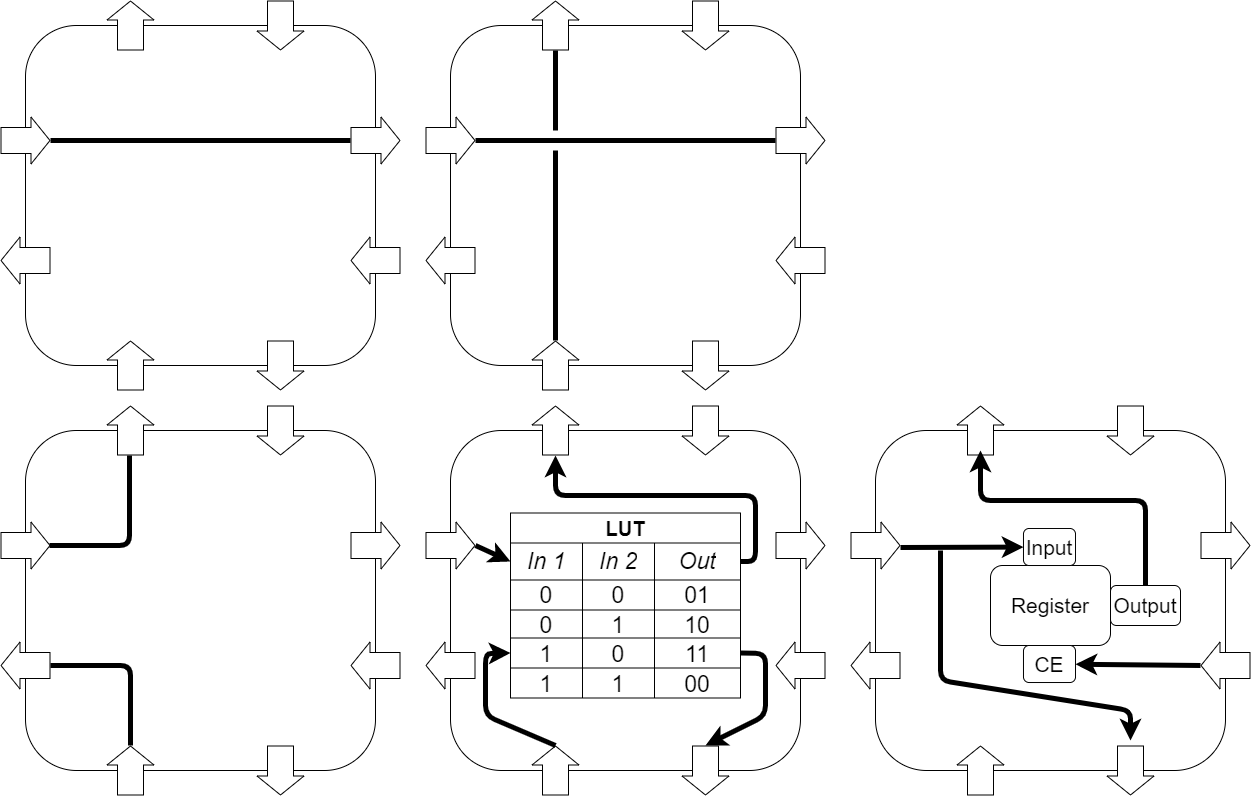
\includegraphics[width=0.8\textwidth]{images/virboard.png}
\caption{All five possible configurations of VirBoard.}
\label{fig:virboardconfigs}
\end{figure}	

There are countless ways to model this functionality using wires, transistors and logic cells, each of which would yield working emulations if a subgraph homeomorphism of the model is found in the graph model of the concrete FPGA. In principle, one could enumerate all such models and attempt to find subgraph homeomorphisms with each of them, maximising the expected result. For the scope of our research, however, we limit ourselves to a single graph model that performs well for subgraph homeomorphism search. For this purpose, we design the model of the virtual FPGA with two goals in mind:

\begin{enumerate}
\item It contains as few vertices and edges as possible, so that the search space is as small as possible.
\item It contains as few rare resources as possible, so that more subgraph homeomorphisms are present.
\end{enumerate}

We designed a graph model of VirBoard that encompasses all listed functionality and contains a total of 30 vertices and 32 edges. We were not able to produce a smaller model or one that uses fewer resources. This graph model of VirBoard is shown in Figure \ref{fig:virboard}.



\begin{figure}
\centering
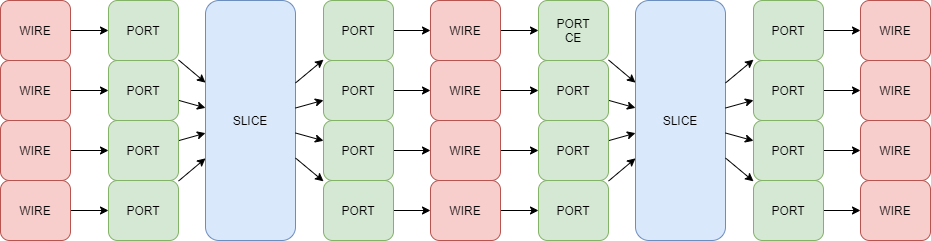
\includegraphics[width=\textwidth]{images/virtualFPGA2.png}
\caption{A graph model of a single cell of the virtual FPGA aimed to emulate on the Lattice ECP5}
\label{fig:virboard}
\end{figure}	

\begin{figure}
\centering
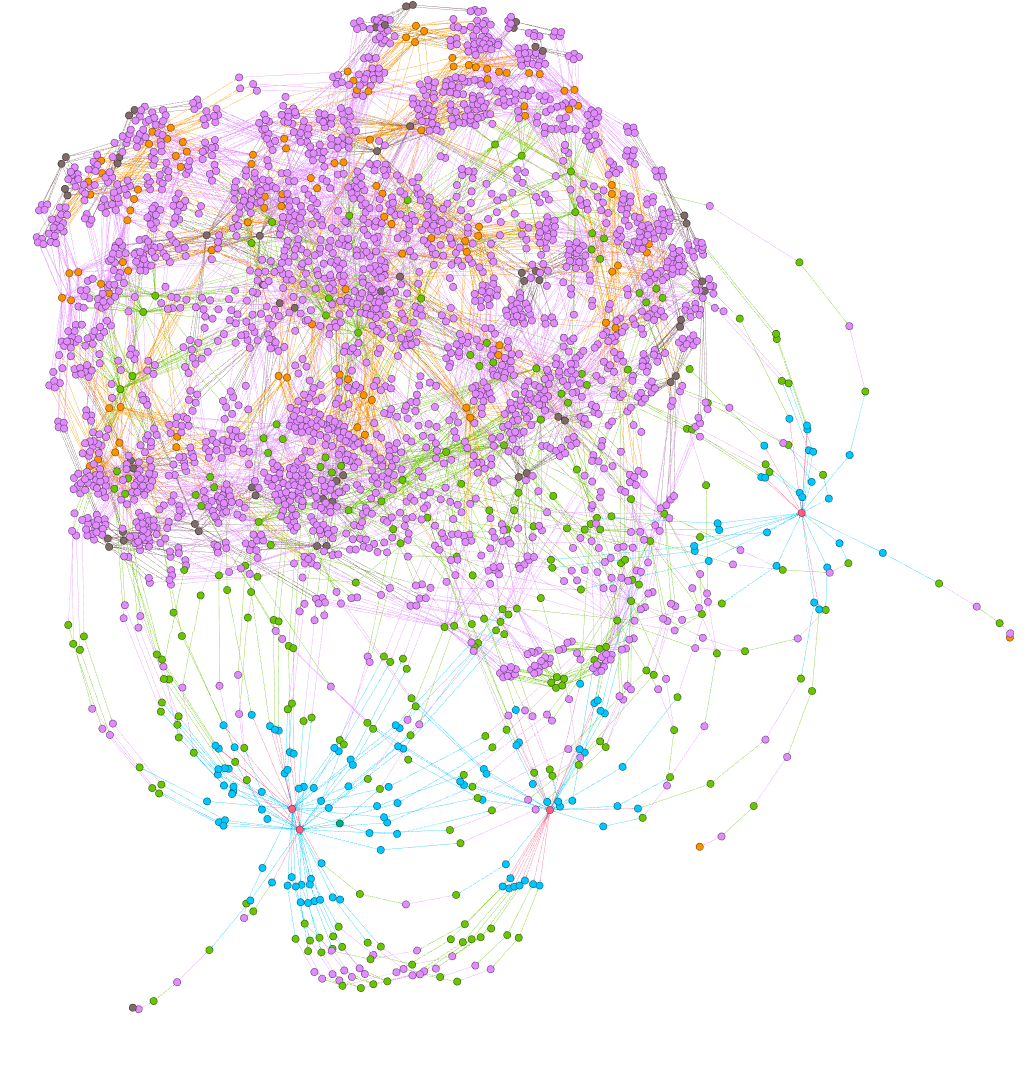
\includegraphics[width=1\textwidth]{images/gephiScreenshot.png}
\caption{Graph model of a single ECP5 logic tile (out of $\pm$42000 logic tiles). Transistors are purple, logical units are red, ports are blue, wires are orange (except those that are neighbouring an adjacent cell, which are brown).}
\label{fig:ECPTGephi}
\end{figure}





\section{Performance experiments}
\section{Software design}
\subsection{Architecture}
\subsection{Manual}
\section{Conclusion}
\section{Discussion}
\section{Future Research}

\begin{appendices}

\section{History of subgraph isomorphism algorithms}
\label{app:algorithmHistory}
\adjincludegraphics[width=\textwidth, trim={0 {.555\height} 0 0},clip]{images/algorithmhistory.png}
\newpage
\adjincludegraphics[width=\textwidth, trim={0 0 0 {.445\height}},clip]{images/algorithmhistory.png}
\section{Examples of path iterators}
\label{app:pathIteratorExamples}
%-----------------
%K-PATH EXAMPLE
%-----------------
\begin{figure}[ht]
\begin{subfigure}{.5\textwidth}
  \centering
  % include first image
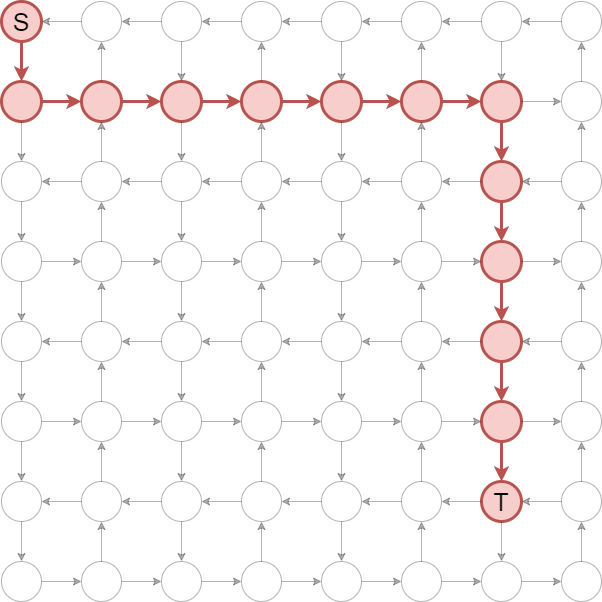
\includegraphics[width=0.8\linewidth]{images/pathiterators/examples-kpath-1.png}
  \caption{First path}
\end{subfigure}
\begin{subfigure}{.5\textwidth}
  \centering
  % include second image
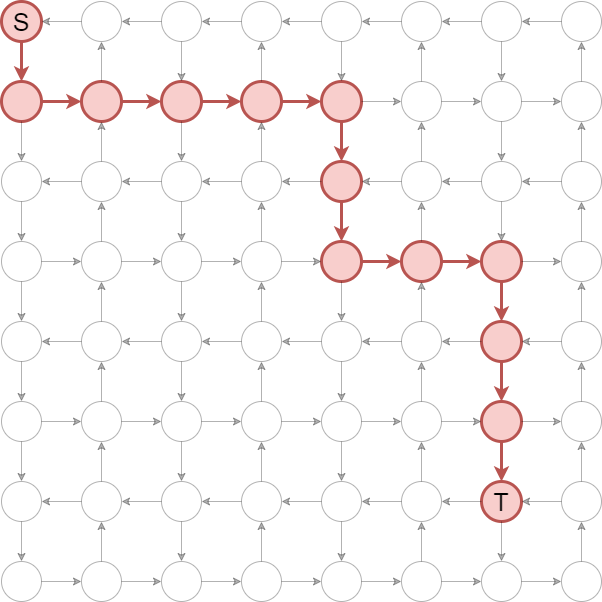
\includegraphics[width=0.8\linewidth]{images/pathiterators/examples-kpath-2.png}
  \caption{Second path}
\end{subfigure}
\caption{The first two iterations of the K-path path iterator in a square graph. This example is unaffected by ``refusing longer paths".}
\label{fig:pathexamples-kpath}
\end{figure}

%-----------------
%DFS EXAMPLE
%-----------------
\begin{figure}[ht]
\begin{subfigure}{.5\textwidth}
  \centering
  % include first image
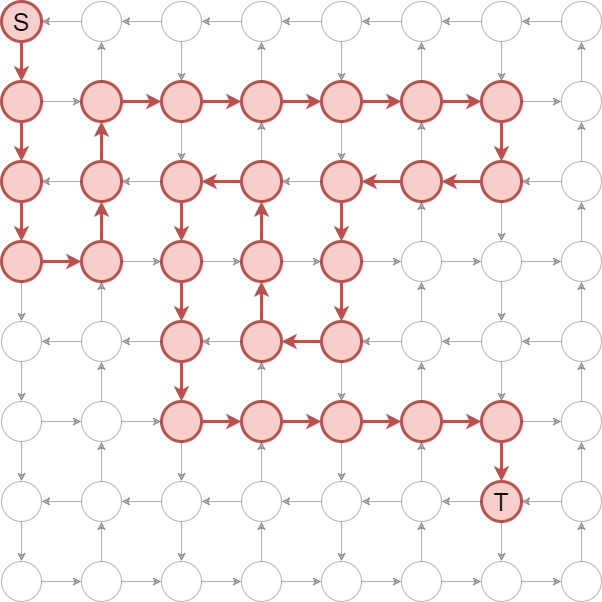
\includegraphics[width=0.8\linewidth]{images/pathiterators/examples-DFS-1.png}
  \caption{First path}
\end{subfigure}
\begin{subfigure}{.5\textwidth}
  \centering
  % include second image
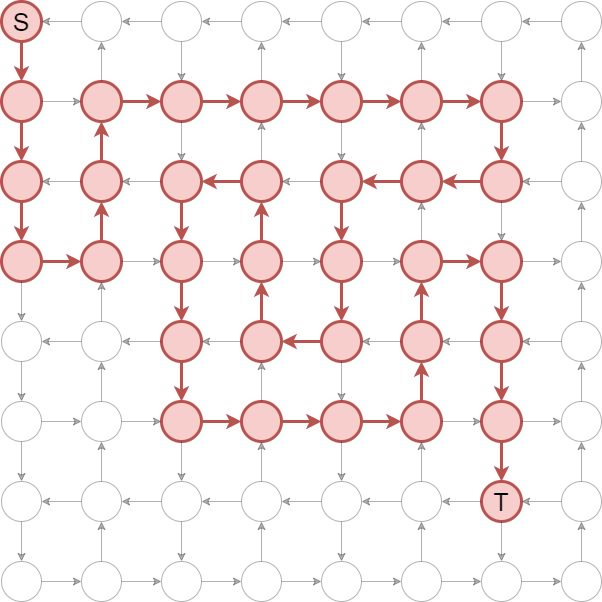
\includegraphics[width=0.8\linewidth]{images/pathiterators/examples-DFS-2.png}
  \caption{Second path}
\end{subfigure}

\begin{subfigure}{.5\textwidth}
  \centering
  % include second image
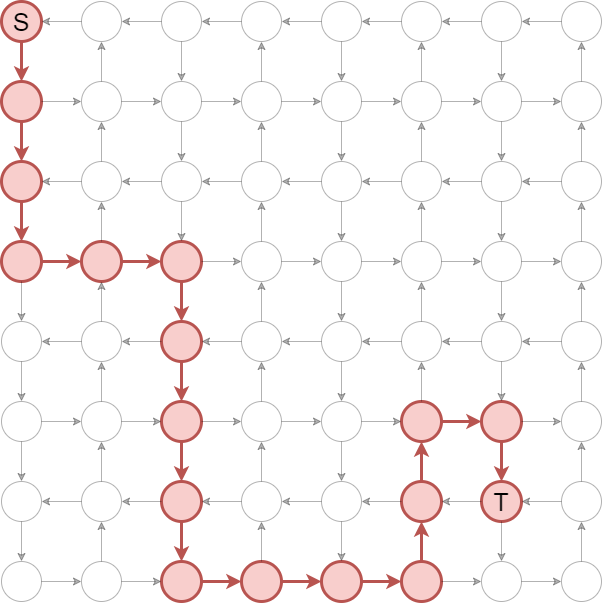
\includegraphics[width=0.8\linewidth]{images/pathiterators/examples-DFS-1-RLP.png}
  \caption{First path (refusing longer paths)}
\end{subfigure}
\begin{subfigure}{.5\textwidth}
  \centering
  % include second image
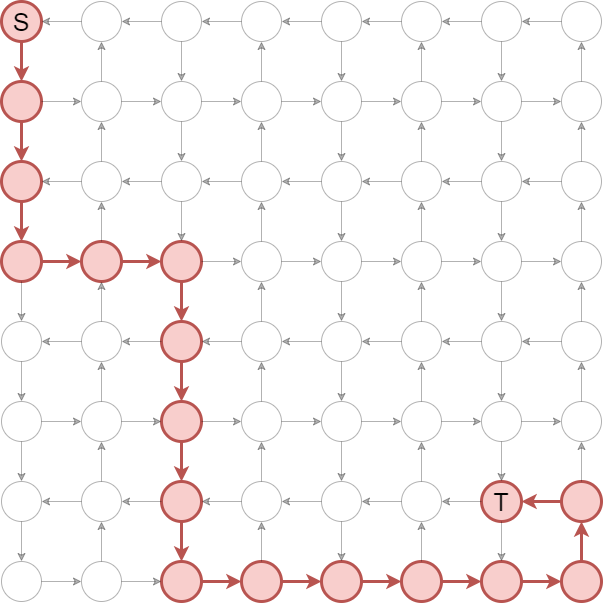
\includegraphics[width=0.8\linewidth]{images/pathiterators/examples-DFS-2-RLP.png}
  \caption{Second path (refusing longer paths)}
\end{subfigure}
\caption{The first two iterations of the DFS path iterator in a square graph.}
\label{fig:pathexamples-dfs}
\end{figure}



%-----------------
%GREEDY DFS EXAMPLE
%-----------------
\begin{figure}[ht]
\begin{subfigure}{.5\textwidth}
  \centering
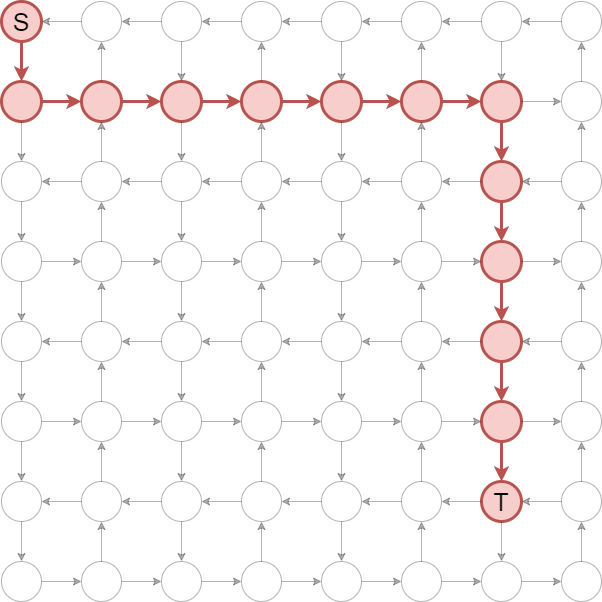
\includegraphics[width=0.8\linewidth]{images/pathiterators/examples-Greedy DFS-1.png}
  \caption{First path}
\end{subfigure}
\begin{subfigure}{.5\textwidth}
  \centering
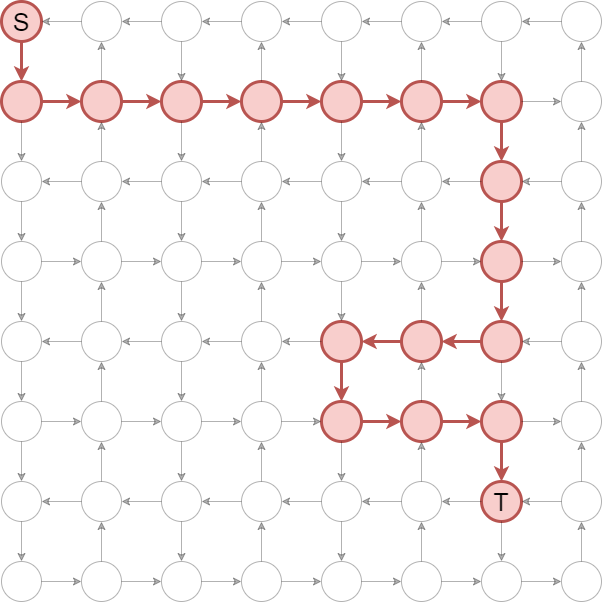
\includegraphics[width=0.8\linewidth]{images/pathiterators/examples-Greedy DFS-2.png}
  \caption{Second path}
\end{subfigure}

\begin{subfigure}{.5\textwidth}
  \centering
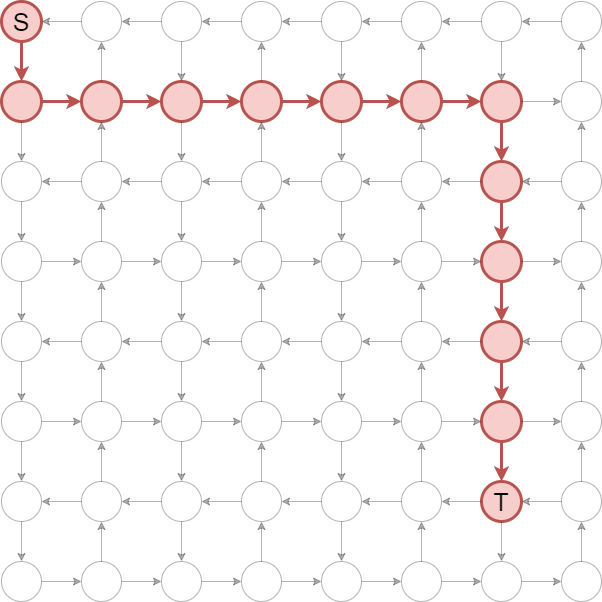
\includegraphics[width=0.8\linewidth]{images/pathiterators/examples-Greedy DFS-1.png}
  \caption{First path (refusing longer paths)}
\end{subfigure}
\begin{subfigure}{.5\textwidth}
  \centering
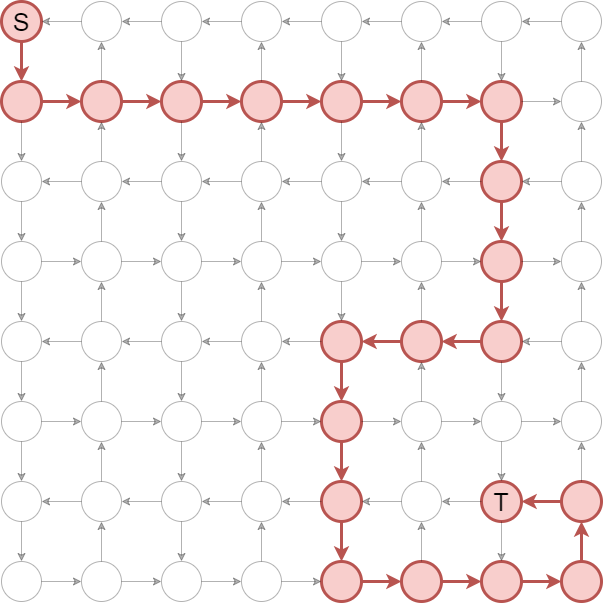
\includegraphics[width=0.8\linewidth]{images/pathiterators/examples-Greedy DFS-reflongerpaths.png}
  \caption{Second path (refusing longer paths)}
\end{subfigure}
\caption{The first two iterations of the greedy DFS path iterator in a square graph.}
\label{fig:pathexamples-greedydfs}
\end{figure}

%-----------------
%CONTROL POINT EXAMPLE
%-----------------
\begin{figure}[ht]
\begin{subfigure}{.5\textwidth}
  \centering
  % include first image
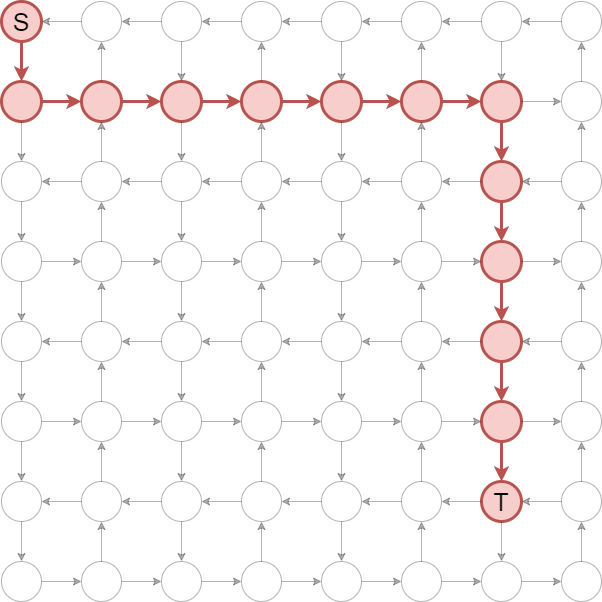
\includegraphics[width=0.8\linewidth]{images/pathiterators/examples-Control point-1.png}
  \caption{First path (0 control points)}
\end{subfigure}
\begin{subfigure}{.5\textwidth}
  \centering
  % include second image
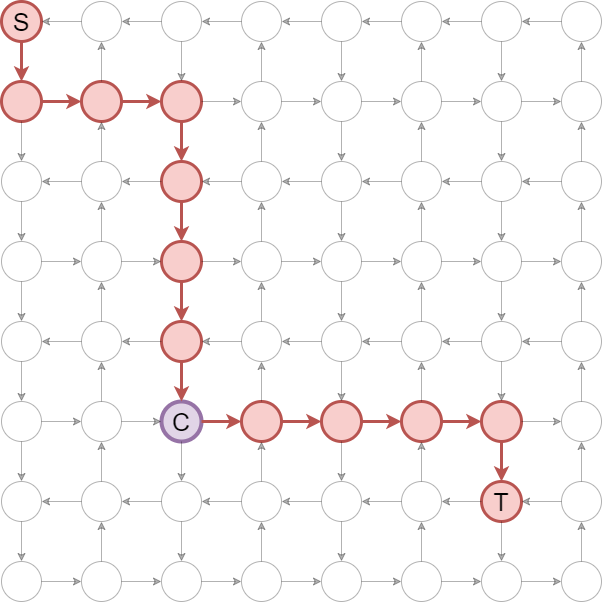
\includegraphics[width=0.8\linewidth]{images/pathiterators/examples-Control point-2.png}
  \caption{Second path (1 control point)}
\end{subfigure}
\caption{The first two iterations of the control point path iterator in a square graph. This example is unaffected by ``refusing longer paths".}
\label{fig:pathexamples-controlpoint}
\end{figure}
\section{Proof: contraction preserves verted disjoint subgraph homeomorphism}
\label{proof:contractionHomeo}
\begin{proof}

Let $M_{V}^{S' to S}$ and $M_{E}^{S' to S}$ be the (injective) vertex-to-vertex mapping and (injective) edge-to-path mapping from $S_{cont}$ to $S$, respectively, and let $(M_{V}^{S to T}, M_{E}^{S to T})$ be some vertex disjoint subgraph homeomorphism from $S$ to $T$, respectively.

We then construct a vertex-to-vertex mapping $M_{V}^{S' to T}$ by mapping each vertex $v \in V_{S'}$ to $M_{V}^{S to T}(M_{V}^{S' to S}(v))$. Recall from the definition of vertex disjoint subgraph homeomorphism that $\forall u \in V_S . L_S(u) \subseteq L_T(M_{V}^{S to T}(u))$. Since for every vertex $v \in V_{S'}$ we have $M_{V}^{S' to S}(v) \in V_s$ (injectivity), it also holds that $\forall u \in V_{S'} . L_S(M_{V}^{S' to S}(u)) \subseteq L_T(M_{V}^{S to T}(M_{V}^{S' to S}(u)))$. Moreover, since labels of remaining vertices are preserved through contraction, we have $\forall v \in V_{S'}.L_{S'}(v)=L_S(M_{V}^{S' to S}(v))$. Therefore, it holds that: $\forall u \in V_{S'} . L_{S'}(u) \subseteq L_T(M_{V}^{S to T}(M_{V}^{S' to S}(u)))$. Therefore, this vertex-to-vertex mapping satisfies the first prequisite out of three for vertex disjoint subgraph homeomorphism.

We then construct an edge-to-path mapping $E_{V}^{S' to T}$. For each edge $(u, v) \in E_{S'}$, we take the edges of the path $M_{E}^{S' to S}(u, v)$ and concatenate the edges of the corresponding paths in $T$ to obtain a new path $p'$. We then add $((u, v), p')$ to $E_{V}^{S' to T}$. Recall from the definition of vertex disjoint subgraph homeomorphism that $\forall(u_1, u_2) \in E_S . \exists p \in values(M_{E}^{S to T}).first(p) = M_{V}^{S to T}(u_1) \land last(p) = M_{V}^{S to T}(u_2) \land ((u_1, u_2), p) \in M_{E}^{S to T}$. 

Since $E_{V}^{S' to T}$ is non-empty, we have $\forall(u_1, u_2) \in E_{S'} . \exists p \in values(M_{E}^{S' to T})$. Moreover, by choosing $p$ for each $(u_1, u_2)$ as $M_{E}^{S' to T}(u_1, u_2)$, we have:

$\forall(u_1, u_2) \in E_{S'} . \exists p \in values(M_{E}^{S' to T}).first(p) = M_{V}^{S' to T}(u_1) \land last(p) = M_{V}^{S' to T}(u_2) \land ((u_1, u_2), p) \in M_{E}^{S' to T}$ which satisfies the second prerequisite.

Lastly, we prove that performing a single contraction does not violate the third prerequisite

$\exists p \in \mathit{values}(M_{E}^{S to T}) . \exists x \in \mathit{intermediate}(p) . \exists p' \in (\mathit{values}(M_{E}^{S to T}) \setminus \{p\}) . x \in \mathit{intermediate}(p')$

and induce that performing any number of contractions does not. Obviously, the base case holds since it is our assumption (i.e. $S$ is vertex disjoint subgraph homeomorphic to $T$). Let $u\in V_S$ have indegree 1 and outdegree 1, qualifying it for contraction. Let the edges be $(\mathit{prec}(u), u)$ and $(u, \mathit{succ}(u))$ where  $\mathit{prec}(u)$ may be equal to $\mathit{succ}(u)$. We know that $M_{E}^{S to T}(\mathit{prec}(u), u)$ is internally vertex disjoint from all other paths in $\mathit{values}(M_{E}^{S to T})$, as well as $M_{E}^{S to T}(u, \mathit{succ}(u))$. They share at least an end vertex $M_{E}^{S to T}(u)$ and possibly $M_{E}^{S to T}(\mathit{prec}(u))$ if $\mathit{prec}(u)=\mathit{succ}(u)$. We know that $M_{E}^{S to T}(u)$ is not the end vertex of another path since $u$ has indegree- and outdegree 1, and not the intermediate vertex of another path since that is not permitted for subgraph homeomorphism. All in all, the combined paths contain intermediate vertices $\mathit{intermediate}(M_{E}^{S to T}(\mathit{prec}(u), u))$, \newline $\mathit{intermediate}(M_{E}^{S to T}(u, \mathit{succ}(u)))$ and the vertex $M_{V}^{S to T}(u)$ that are not intermediate vertices of other paths in $values(M_{E}^{S to T})$.

When we contract this vertex, we get a new edge $(\mathit{prec}(u), \mathit{succ}(u))$ with start vertex $M_{E}^{S to T}(\mathit{prec}(u))$, end vertex $M_{E}^{S to T}(\mathit{succ}(u))$, and as intermediate vertices \newline $\mathit{intermediate}(M_{E}^{S to T}(\mathit{prec}(u), u)) \cup \mathit{intermediate}(M_{E}^{S to T}(u, \mathit{succ}(u))) \cup M_{V}^{S to T}(u)$. The vertex set used in $T$ remains exactly the same, thus does still not share intermediate vertices with other paths in $values(M_{E}^{S to T})$.
 
By induction, the third prerequisite holds. Since all prerequisites hold, $S'$ is a vertex disjoint subgraph homeomorphism of $T$.


%
%Then, $x$ is part of the middle section of at least two different paths in $T$. Let us call these paths $p_1$ and $p_2$. These paths were concatenated from \textit{vertex disjoint} paths in $\mathit{values}(M_{E}^{S to T})$. This implies that ${M_{E}^{S to T}}^{-1}(x)$ (let us call this $x'$) must be a contracted vertex. Therefore, there exists some path segment $p_1' \in \mathit{values}(M_{E}^{S to T})$ that contains $x$ as end vertex and some path segment $p_1''\in \mathit{values}(M_{E}^{S to T})$ that contains $x$ as start vertex, and similarly for $p_2'$ and $p_2''$. Then, at least one of the following is true:
%
%\begin{itemize}
%\item $x'$ has at least indegree 2 in which case we have a contradiction, since $x'$ was contracted.
%\item $x'$ has at least outdegree 2 in which case we have a contradiction, since $x'$ was contracted.
%\item $x'$ has a predecessor $prec(x')$ and successor $succ(x')$ such that $M_{E}^{S to T}(prec(x'))$
%\end{itemize}
%
%$x'$ has at least indegree 2 or outdegree 2 or $p_1$ and $p_2$ share . However, we deduced that $x'$ must have been contracted, which is not performed on vertices with these indegrees and outdegrees.
%
%Since our assumption leads to a contradiction, we have proven its negation which is $\forall p \in \mathit{values}(M_{E}^{S' to T}) . \forall x \in \mathit{intermediate}(p) . \not \exists p' \in (\mathit{values}(M_{E}^{S' to T}) \setminus \{p\}) . x \in \mathit{intermediate}(p')$ which satisfies the third prerequisite.
\end{proof} 


\end{appendices}


\newpage
\printbibliography

\end{document}
